
\chapter{Results}

In this chapter, different approaches for training the YOLO model are presented. First, the results of training a simple large model will show a baseline model which is then improved by different settings. Afterwards, the results of training the small and medium model are shown. Finally, the three different model sizes are compared.

\section{Large Network}

The first experiments were made with only a small part of the data set being manually labeled. At first, the images of the TUM data that contain approximately one big sugar beet per image were labeled automatically with \texttt{0 0.5 0.5 1 1}. This means that the whole picture is labeled as containing exactly one sugar beet. We assumed that these images were already in the perfect format for our use case and the automatic labeling would be sufficient. The images containing multiple small plants are labeled manually and exactly. The model was trained with default hyperparameters and settings. This means that the number of epochs is 300, box loss gain of 0.05, class loss gain of 0.5, object loss gain of 1.0 and IoU threshold for training of 0.2. The data augmentation values can be found in table \ref{tab:augmentation_exp1}.

\begin{table}[h!]
	\centering
	\begin{tabular}{|c c c c c c c c c c c c c|} 
		\hline
		Hue & Sat & Val & Deg & Trans & Scale & Shear & Persp & UD & LR & Mos & Mix & CP\\ % [0.5ex]  
		\hline
		0.015 & 0.7 & 0.4 & 0.0 & 0.1 & 0.5 & 0.0 & 0.0 & 0.0 & 0.5 & 1.0 & 0.0 & 0.0 \\
		\hline
	\end{tabular}
	\caption{Values for data augmentation. Hue, Saturation and Value are given in a fraction. Deg is degree of the rotation, Trans the translation (fraction), scale and shear (also in degree). UD and LR are the probabilities of the image to be flipped up-down (UD) or left-right (LR). Mosaic, mixup and copy paste are also given as probabilities. }
	\label{tab:augmentation_exp1}
\end{table}

All in all, small data augmentation is used. $ 85\% $ of the data was used as training set and $ 15\% $ as validation set. The different image types were divided equally into each set (training and validation).\\


For the training and validation set, the results were accurate. With a real number of 9110 sugar beets and a detected number of plants of 8162, this results in an accuracy of $ 89,6\% $. Although for new, unseen images, the accuracy is very low. Here, the number of labeled sugar beets is 575 and only 68 are detected. An overall accuracy of $ 11,8\% $ results. In this experiment, only the number of detected and real sugar beets are observed, not the location or size of the bounding boxes. However, the results show that this model is not sufficient for detecting the boundaries of sugar beets. Two examples of detected objects can be seen in figure \ref{fig:results_experiment_1}.

\begin{figure}[htb!]
	\centering
	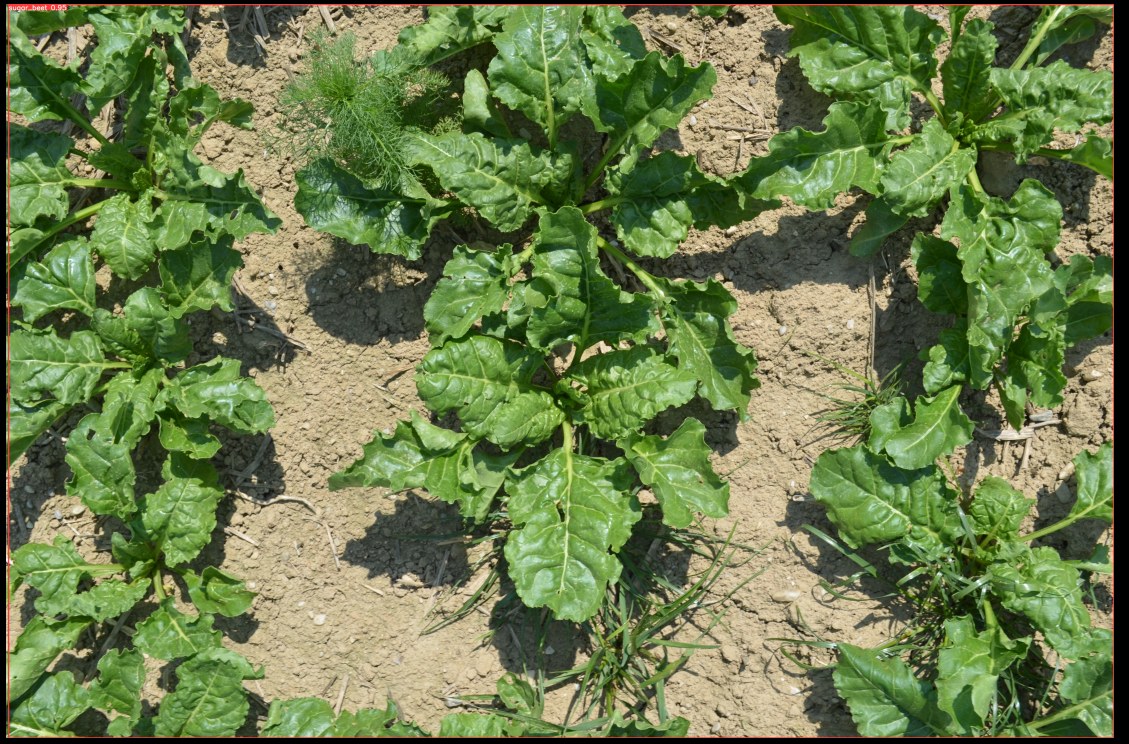
\includegraphics[scale=0.178]{figures/results_exp1_1.png}
	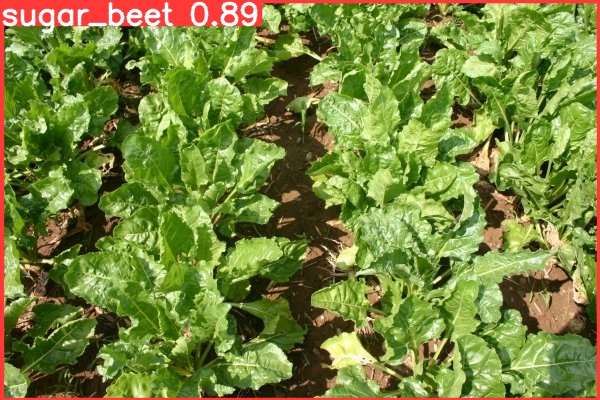
\includegraphics[scale=0.33]{figures/results_exp1_2.JPEG}
	\caption{Examples of whole images being detected as one sugar beet. That was one of the problems that had to be faced.}
	\label{fig:results_experiment_1}
\end{figure}

You can see that in both cases, the whole image is detected as one plant. In the left example, the angle of the recording camera is very good with $ 90° $, in the right example which is taken from the Imagenet folder containing sugar beet images, the angle is not perfect. However, also here the whole images is labeled as sugar beet. the class probabilities are $ 0.95 $ in the left case and $ 0.89 $ in the right image.\\

Another problem of this model is the high false positive rate in case of other plants. In another test, 1271 images of all kinds of plants of Imagenet are tested. 922 labels of sugar beets were detected which means that about $ 70\% $ are detected false positive. Two examples can be seen in figure \ref{fig:false_positives}.

\begin{figure}[htb!]
	\centering
	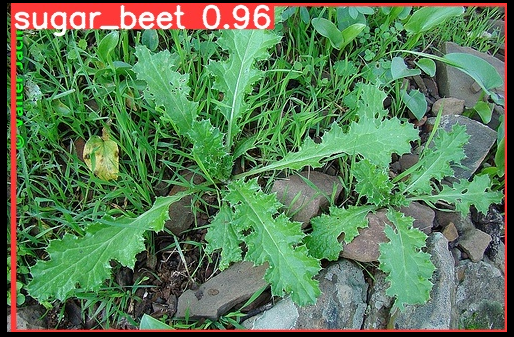
\includegraphics[scale=0.458]{figures/false_positive_1.png}
	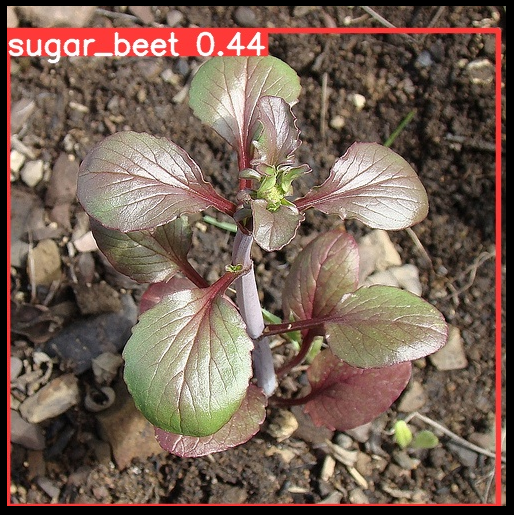
\includegraphics[scale=0.3]{figures/false_positive_2.png}
	\caption{Examples of other plants also detected as sugar beets. That was another problem that had to be solved.}
	\label{fig:false_positives}
\end{figure}

You can see that also random plants are detected as sugar beets which should not be the case.\\

The following figure \ref{fig:AUC_comparison} shows the testing result of different training strategies and setting to mitigate this problem.

\begin{figure}[htb!]
	\begin{subfigure}{.5\textwidth}
		\centering
		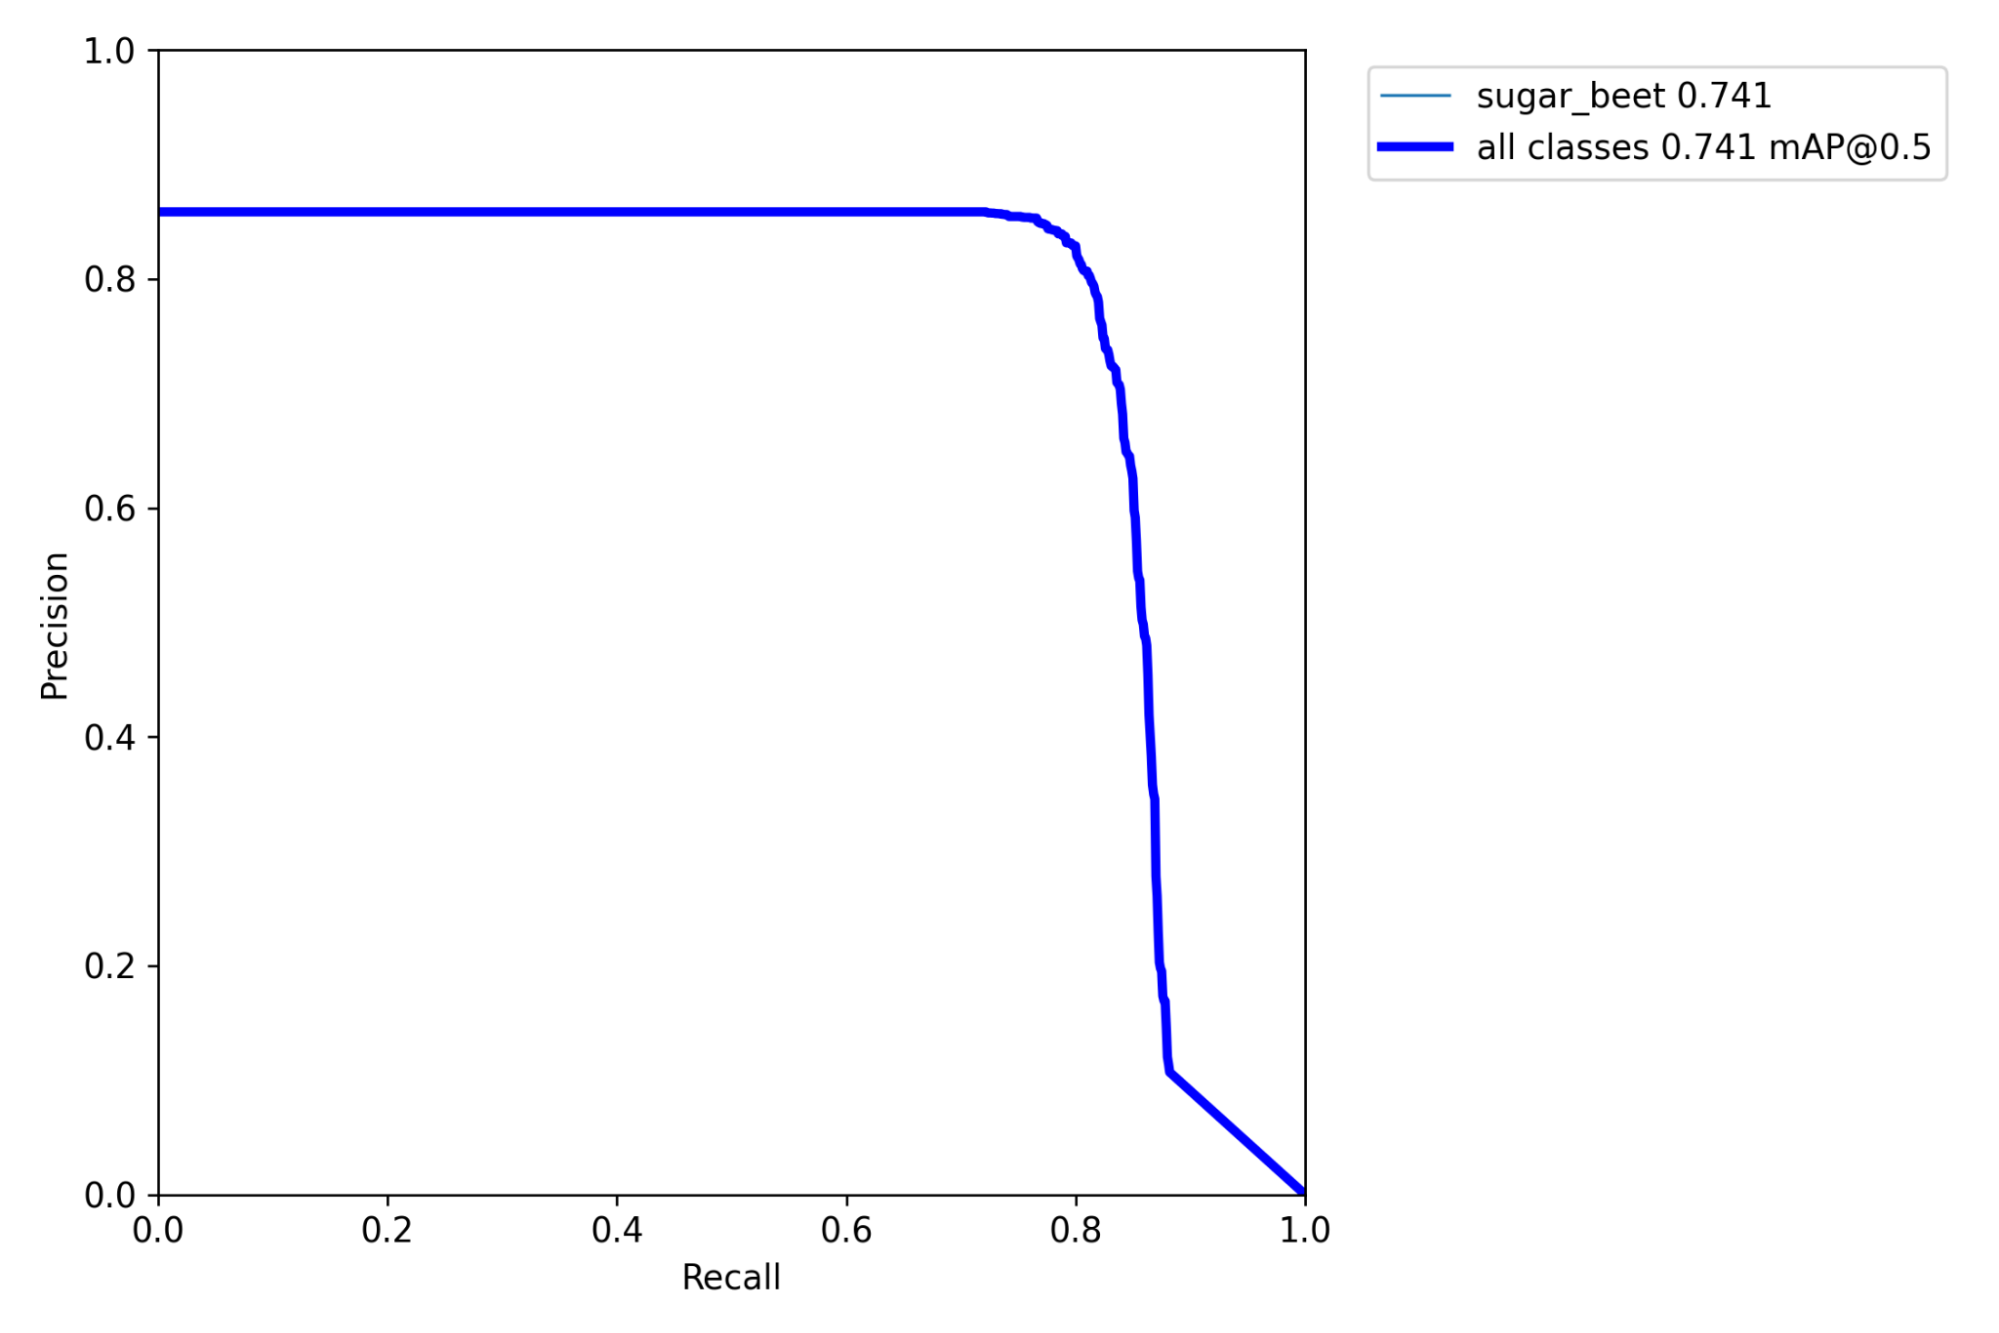
\includegraphics[scale=0.08]{figures/exp1_curve.png}
		\caption{P-R-curve for the first experiment. With mainly automatically labeled images, an average precision of only 0.741 can be achieved.}
		\label{fig:AUC_1}
	\end{subfigure}%
	\begin{subfigure}{.5\textwidth}
		\centering
		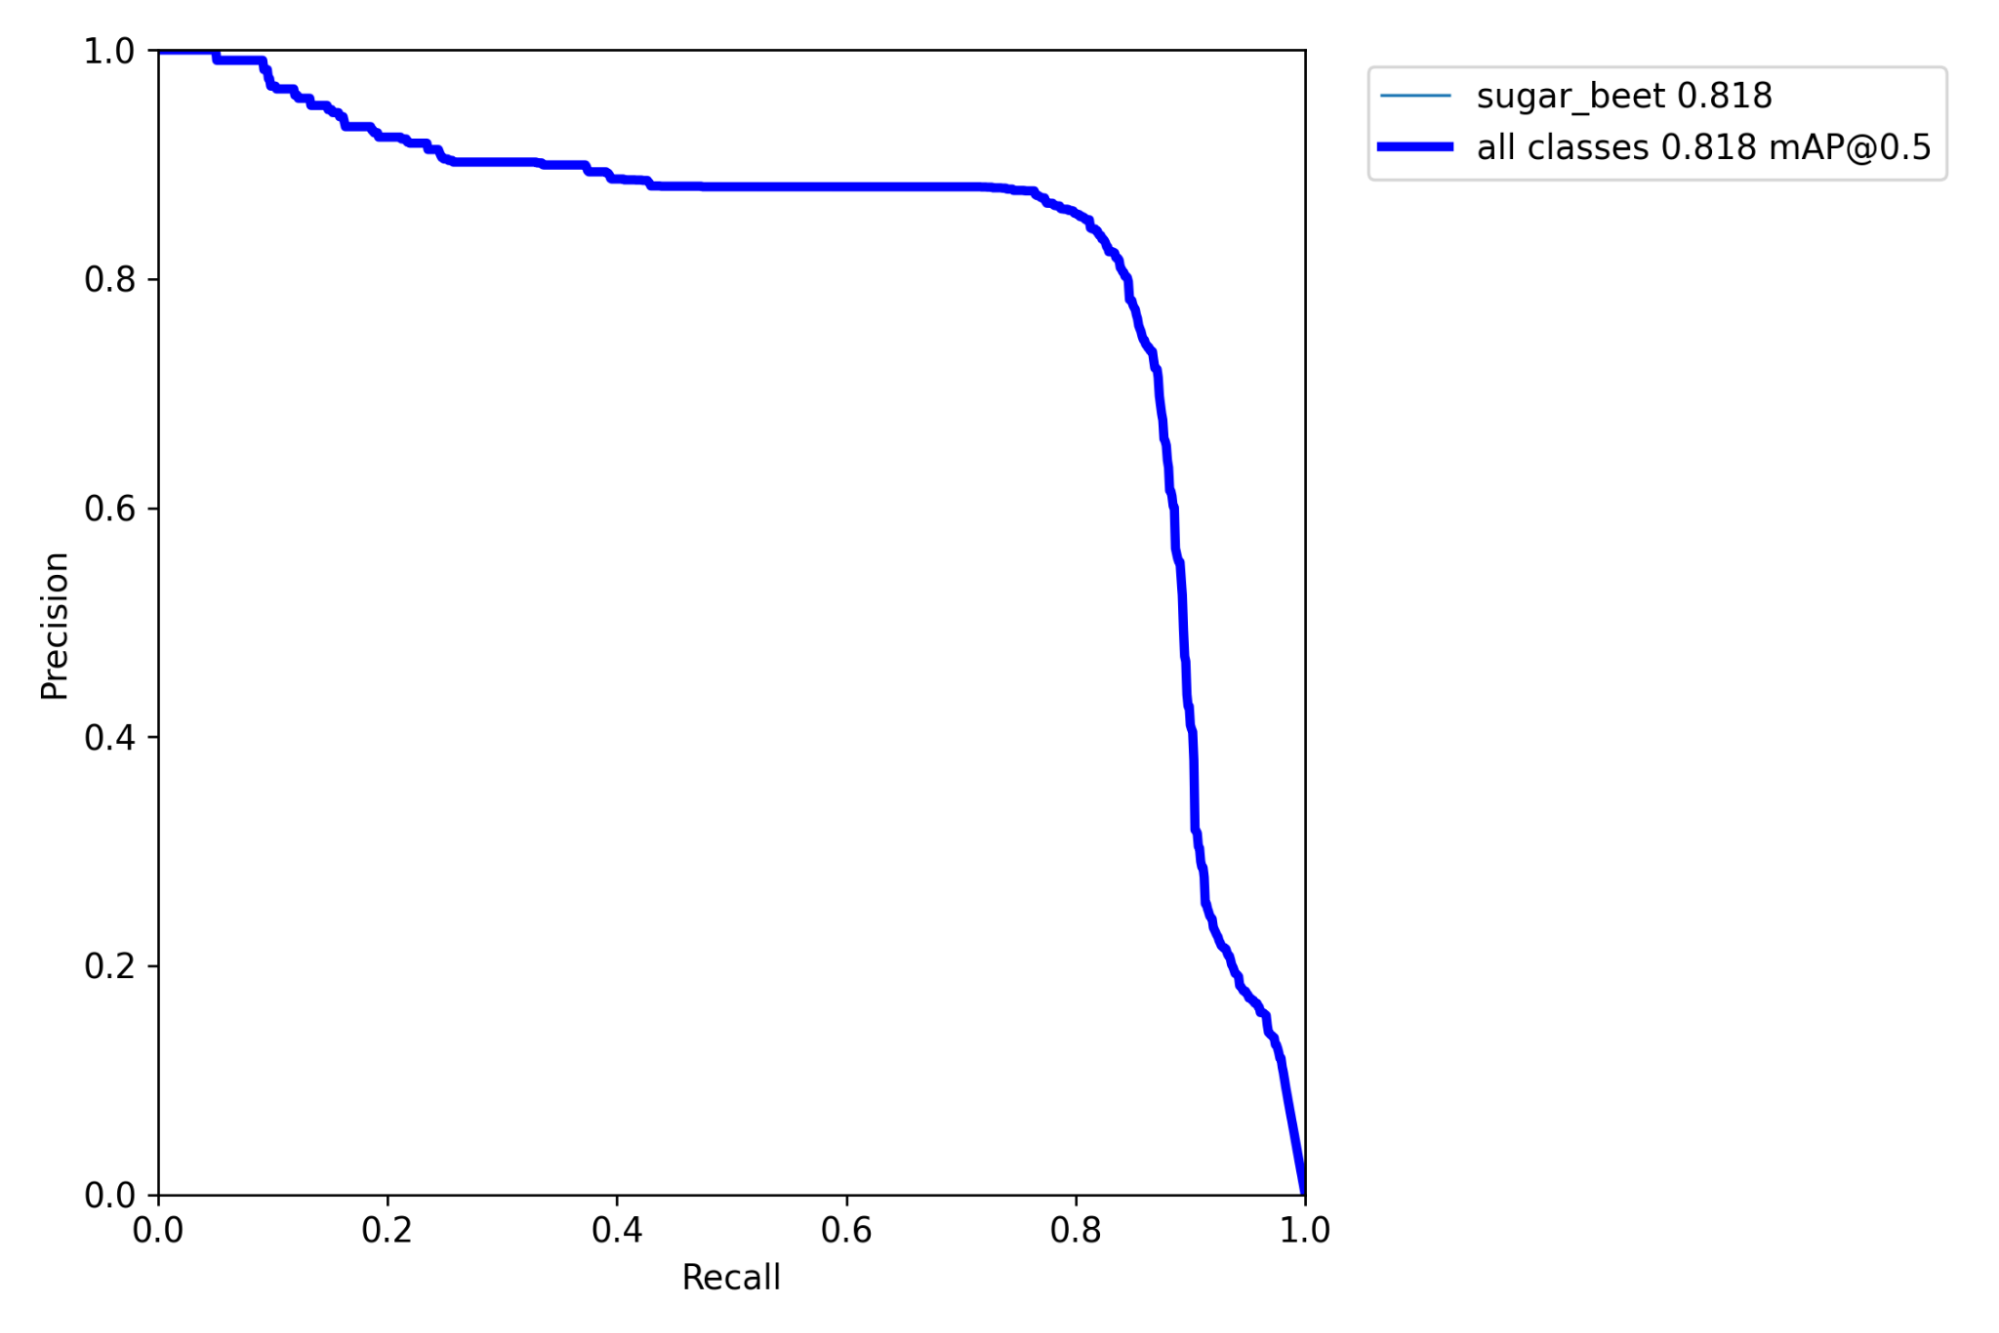
\includegraphics[scale=0.08]{figures/no_pre_low_dat.png}
		\caption{P-R-curve for the second experiment. Now, the AUC has increased to 0.818 by adding manually labeled images. }
		\label{fig:AUC_2}
	\end{subfigure}
	\begin{subfigure}{.5\textwidth}
		\centering
		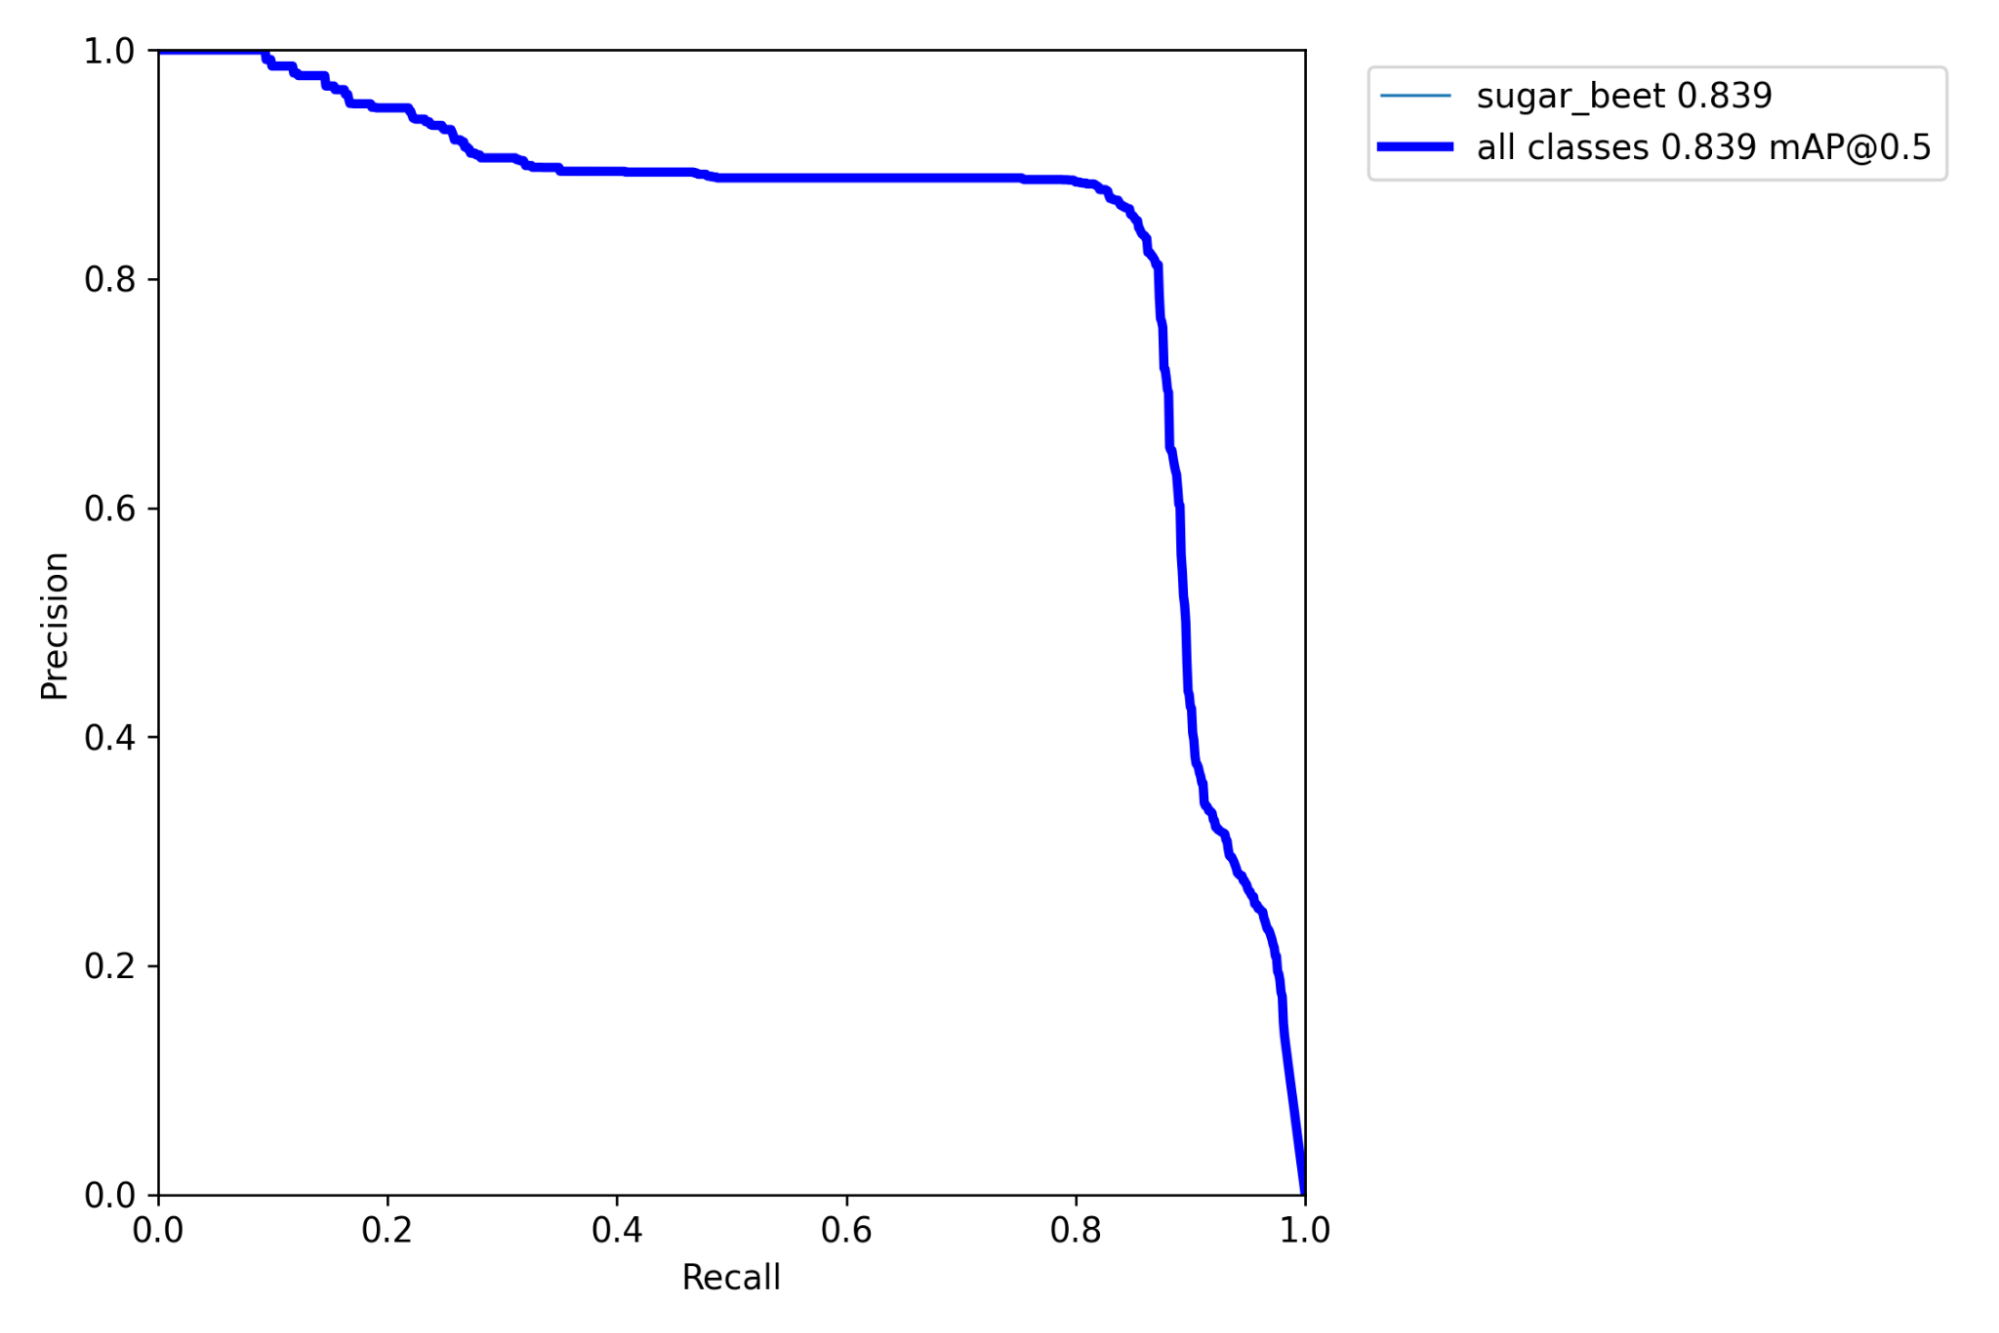
\includegraphics[scale=0.08]{figures/no_pre_high_dat.png}
		\caption{P-R-curve of third experiment. Now, higher data augmentation is used, leading to higher AUC of 0.839.}
		\label{fig:AUC_3}
	\end{subfigure}
	\begin{subfigure}{.5\textwidth}
		\centering
		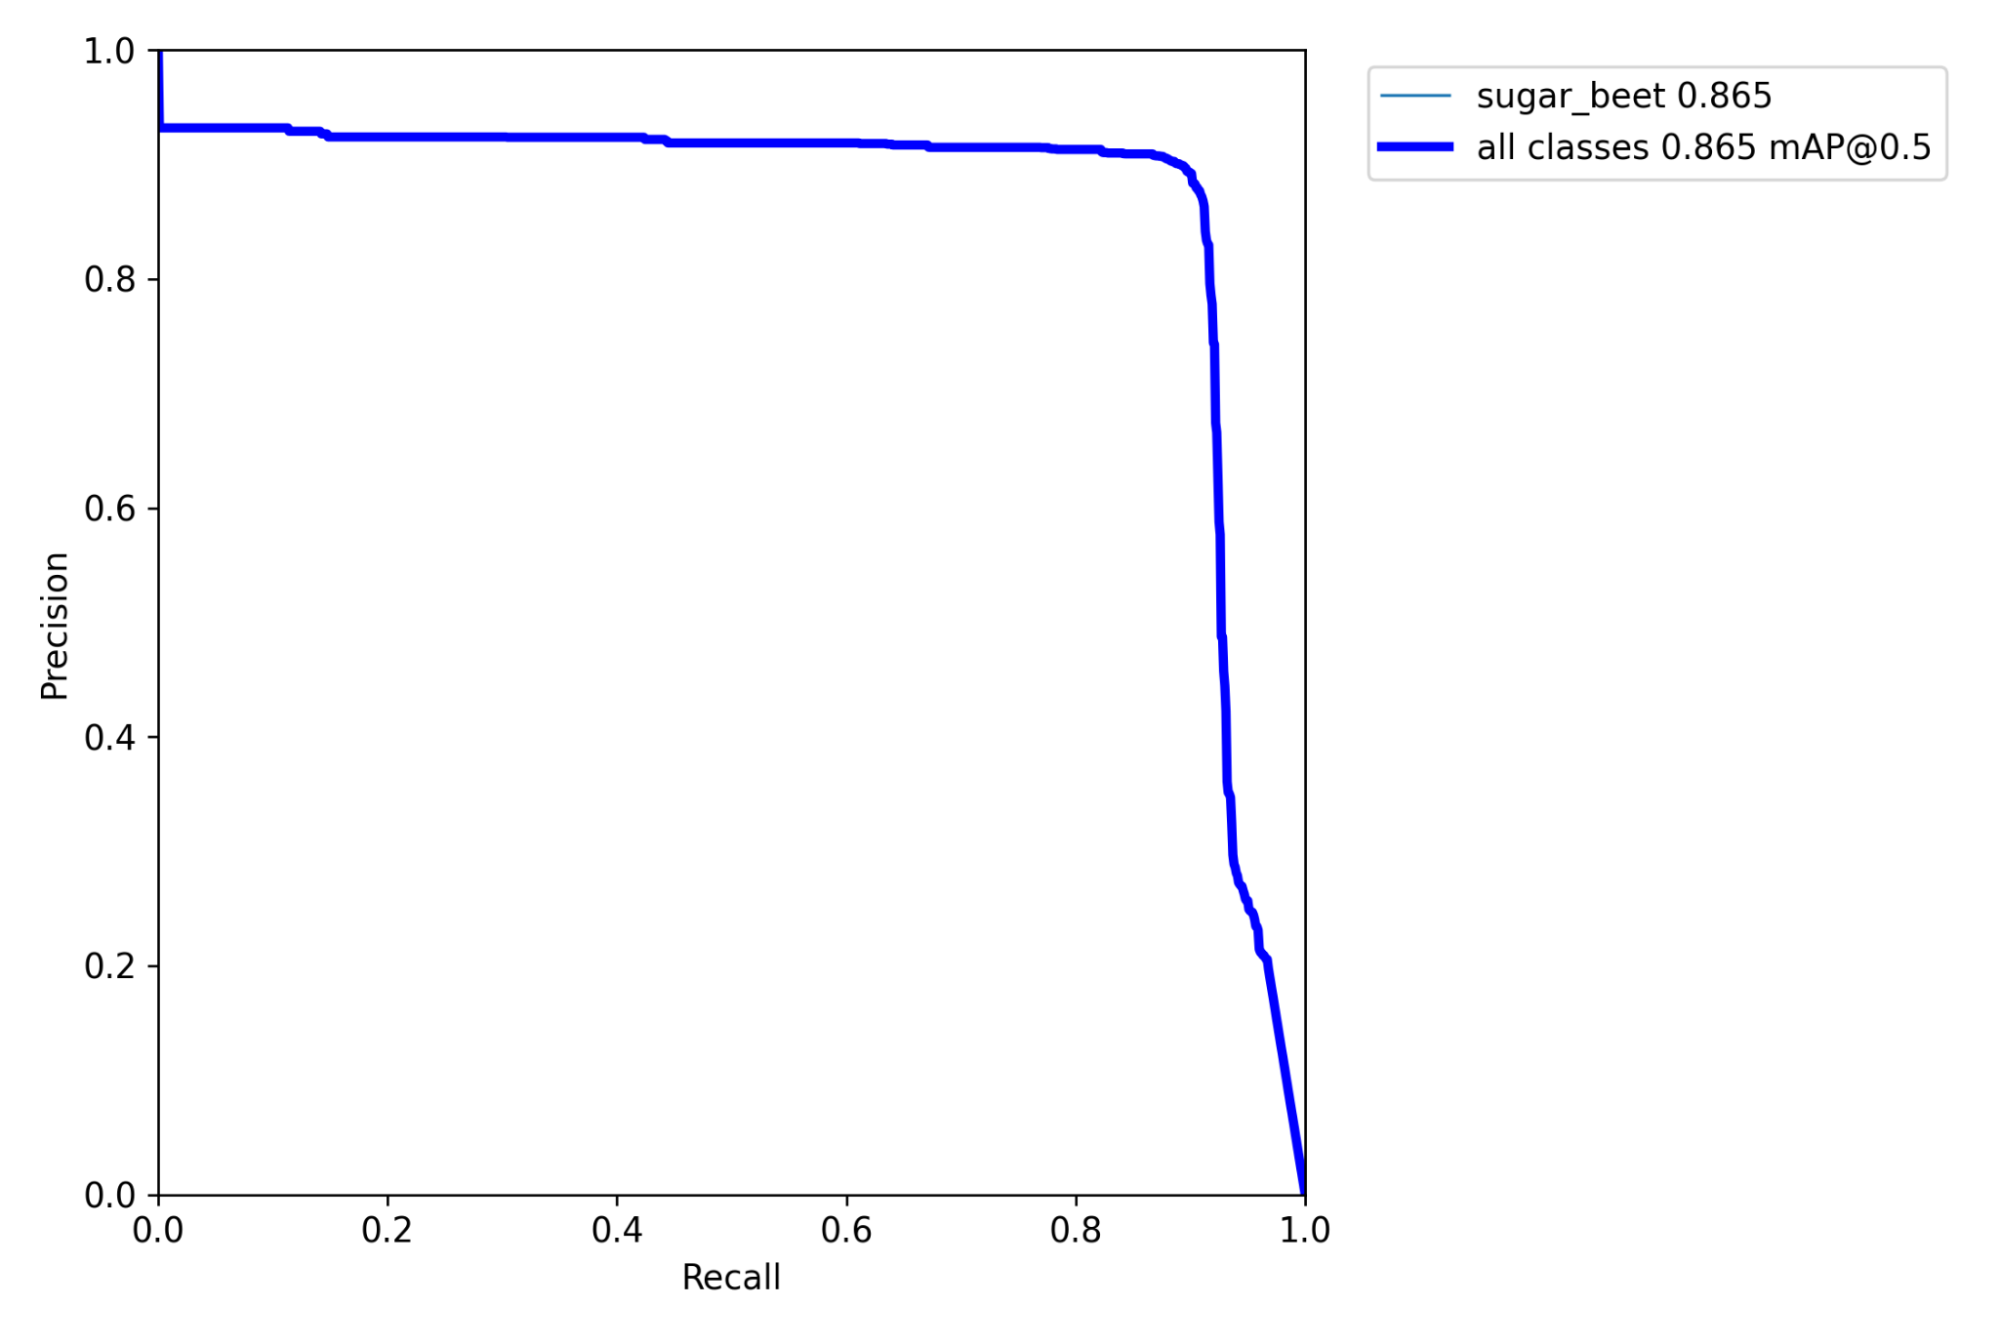
\includegraphics[scale=0.08]{figures/yes_pre_low_dat.png}
		\caption{P-R-curve of fourth experiment. Now, the training was done with two classes (also other\_plant). The resulting AUC is 0.865.}
		\label{fig:AUC_4}
	\end{subfigure}
	\begin{subfigure}{1\textwidth}
		\centering
		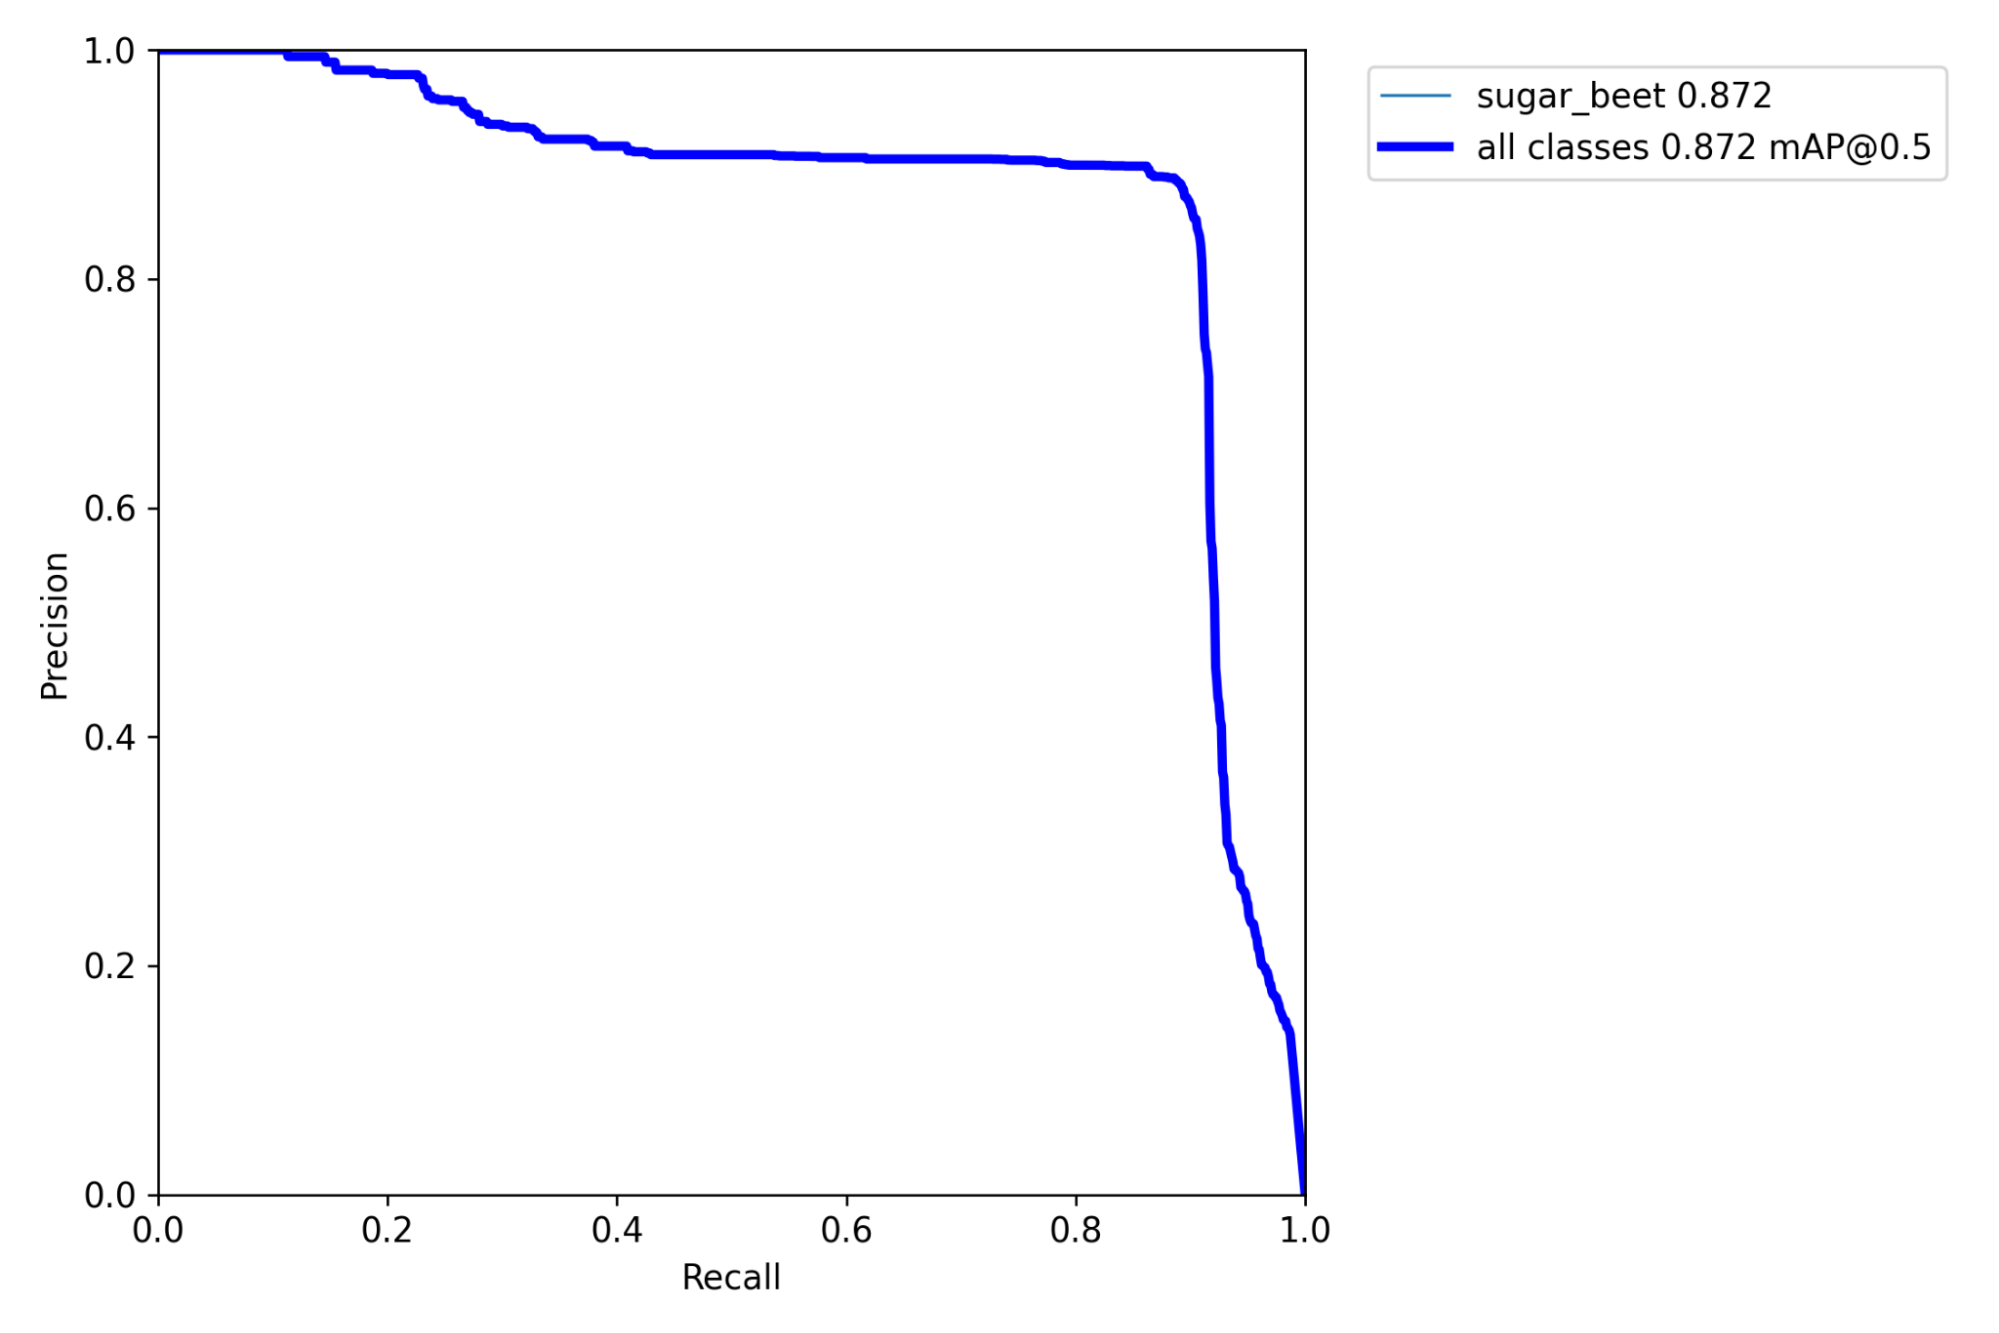
\includegraphics[scale=0.08]{figures/yes_pre_high_dat.png}
		\caption{P-R-curve of last experiment. With only one class and higher data augmentation, an average precision of 0.872 can be achieved.}
		\label{fig:AUC_5}
	\end{subfigure}
	\caption{Comparison of testing P-R-curves of the different training experiments.}
	\label{fig:AUC_comparison}
\end{figure}

Testing the model with a test set consisting of the heterogeneous Partner data and 400 TUM images which contain multiple small plants and also larger ones, yields the following result which can be seen in figure \ref{fig:AUC_1}.

A perfect model would have an area under curve of $ 1.0 $. This one has $ 0.741 $ which still has room for improvement.\\


All in all, we encounter two main problems. The first one is that the bounding boxes of detected plants are just very inaccurate. Most of the time, the whole image is labeled as one sugar beet. The second problem is that the model is not robust. It also detects other plants as sugar beets and it can not distinguish between different kinds of plants.

The first problem can be solved by labeling the data more accurate. By this, the model learns the exact boundaries of sugar beet plants and the predicted results get better. For the second problem, two different solutions exist. One is to add another class called other plant which is essentially everything else than sugar beets. The problem of this is that for example cars or persons are also detected as other plant which is also not intended. The second possible solution of this problem is to add so called background images. These are pictures which are not labeled with any object. Possible images therefore are other plants, persons or cars. At first, we added the so called other\_plant class to get a better distinction between sugar beets and any different type of plant. \\

Although the predicted results are not too good by now, the model has already seen the structures of sugar beets. This can be used as pretrained model. In the following, four different training strategies are presented. The goal is to compare training the model from scratch and using the pretrained version. Additionally, the impact of including background images is investigated. The values of different hyperparameters for higher data augmentation can be seen in table \ref{tab:high_augmentation}.

\begin{table}[h!]
	\centering
	\begin{tabular}{|c c c c c c c c c c c c c|} 
		\hline
		Hue & Sat & Val & Deg & Trans & Scale & Shear & Persp & UD & LR & Mos & Mix & CP\\ % [0.5ex] 
		\hline
		0.015 & 0.7 & 0.4 & 0.0 & 0.1 & 0.9 & 0.0 & 0.0 & 0.0 & 0.5 & 1.0 & 0.1 & 0.1\\
		\hline
	\end{tabular}
	\caption{Values for higher data augmentation. Meanings of the variables are the same as in \ref{tab:augmentation_exp1}. Now, higher values are used compared to the first one.}
	\label{tab:high_augmentation}
\end{table}

The first experiment is done from scratch without pretraining and lower data augmentation. The dataset used is labeled completely by hand. The results of the tests can be seen in figure \ref{fig:AUC_2}.


With an AUC (area under curve) of $ 0.818 $, it has already better results compared to the first experiment. The reason is the more exact labeling. \\

In the next training, again no pretrained model was used. Instead, the parameters were adjusted to use higher data augmentation. The results of the testing can be seen in figure \ref{fig:AUC_3}.


You can see that an improvement can be achieved with an AUC of $ 0.839 $ (compare $ 0.818 $ from before). We can conclude from this that data augmentation has quiet a high impact on the accuracy. \\

In the next experiment, the pretrained model from before is used. The data augmentation is again the higher one and here, the images of other plants from Imagenet are labeled with other\_plant. Testing results can be seen in figure \ref{fig:AUC_4}.

With an AUC of $ 0.865 $, the prediction accuracy again has improved. \\

In the next experiment, the difference to the previous one is that the images from Imagenet are not labeled at all. As already mentioned, the problem of the inexact labeling of the Imagenet pictures can sometimes lead to unintended predictions. The testing results of this experiment can be seen in figure \ref{fig:AUC_5}.

This model has the best AUC with $ 0.872 $.\\


The accuracy measured in AUC of the P-R-curve, improved with the different training settings. Figure \ref{fig:direct_comparison} visualizes this again. There, the average precisions of each model are compared. 

\begin{figure}
	\centering
	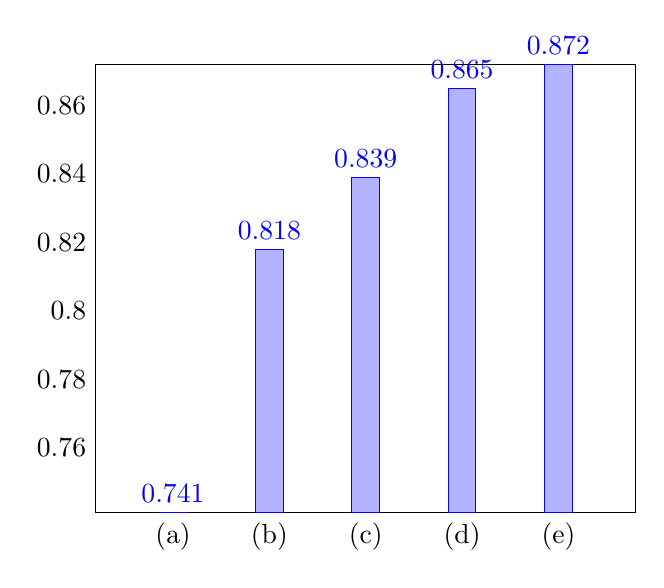
\begin{tikzpicture}
	\begin{axis} 	 [
	ybar,
	tickwidth         = 0pt,
	enlarge x limits  = 0.2,
	enlarge y limits  = 0.0002,
	nodes near coords={\pgfmathprintnumber[precision=4]{\pgfplotspointmeta}},
	%nodes near coords,
	symbolic x coords = {(a), (b),
		(c), (d), (e)},
	]
	\addplot coordinates { ((a),0.741) ((b),0.818)
		((c),0.839) ((d),0.865) ((e),0.872) };
	\end{axis}
	\end{tikzpicture}
	\caption{Direct comparison of the average precision of the different training experiments. At first, the AUC increases fast. A saturation can be seen at the last experiments.}
	\label{fig:direct_comparison}
\end{figure}

It can be observed that the best improvement is made with the exact labeled data. In general, the precision gets better with different training settings and techniques, but the difference between them decreases. This might be a saturation where no big improvements can be made anymore. \\

Now with these improvements, the new predictions are more accurate and also, the problem of the second class other\_plant is no longer existent. Examples for current predictions can be seen in figure \ref{fig:current_predictions}.

\begin{figure}[htb!]
	\centering
	\includegraphics[scale=0.2]{figures/pred1.png}
	\includegraphics[scale=0.2]{figures/pred2.png}
	\caption{Predictions of sugar beets in screenshots of drone videos. Now, single plants are detected with high accuracy of bounding boxes. }
	\label{fig:current_predictions}
\end{figure}

These predictions were made in one of the drone videos. You can see that now, the bounding boxes are just around one plant each. This is the behavior that was expected of the object detection algorithm. Previously, the whole image or one row of plants were labeled as sugar beets. Other problems like detecting the image as other\_plant if no sugar beet was detected is also improved. 

\section{Small and Medium Network}

As already mentioned, the inference time of the large model don't really make it possible to apply it in the application in-place. This is the reason why also the small and medium sized model is trained. Already some behavior could be seen in experiments with the large model such as the improvements of including exactly labeled images, background data with no labels and using higher data augmentation. The results of the small and medium sized models are presented in the following. \\

First experiments are made with the models which are pretrained using the COCO dataset. Data augmentation was low and also all other hyperparameters were chosen to be the default ones as this was just a first experiment to compare the accuracy of the two types of models. Figure \ref{fig:comparison_small_medium} depicts the testing results. 

\begin{figure}[htb!]
	\centering
	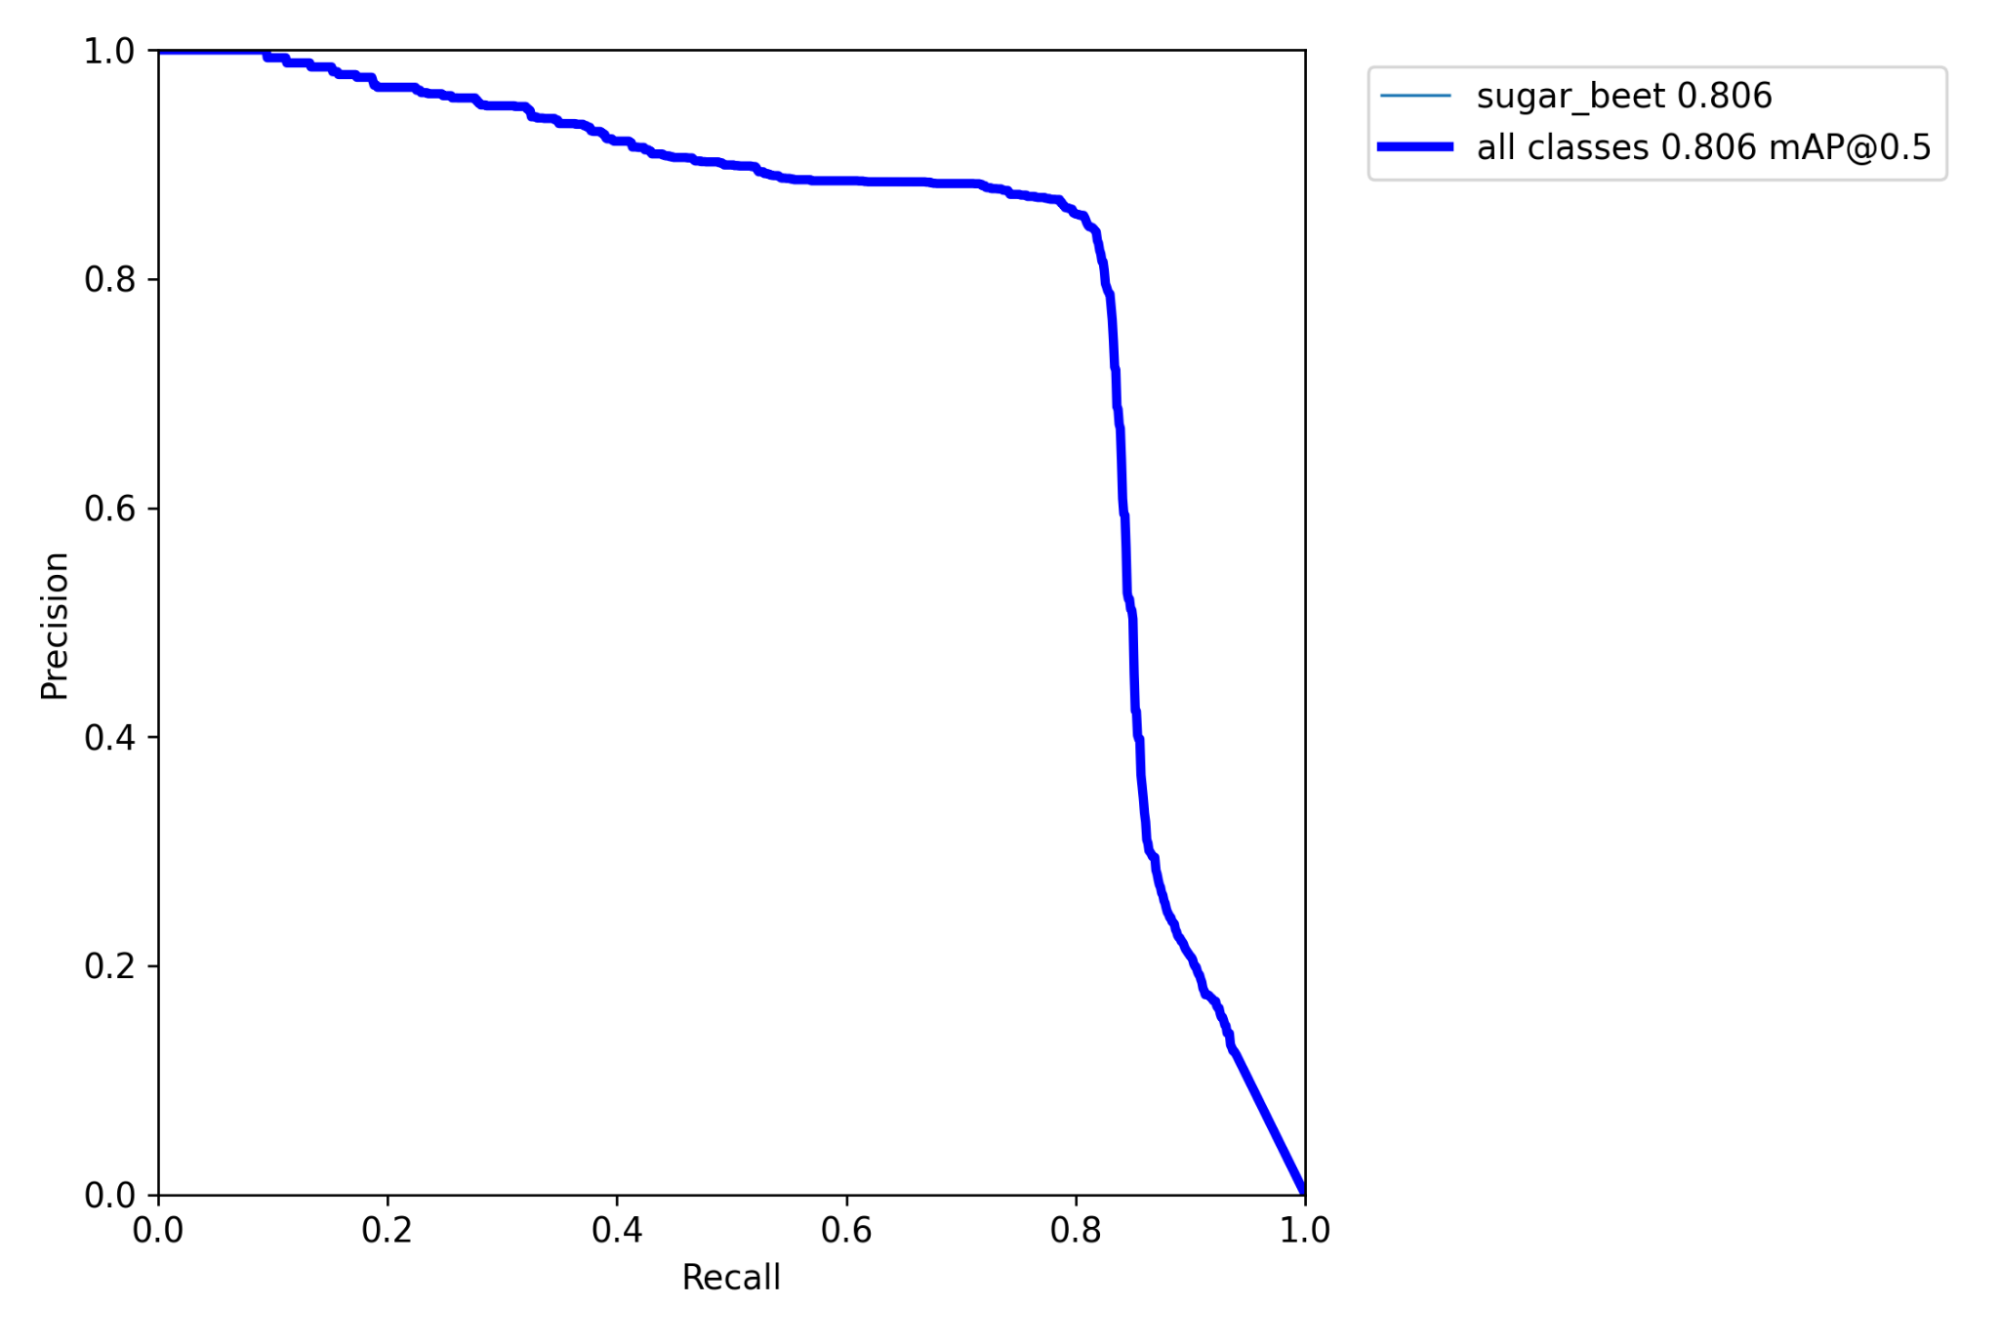
\includegraphics[scale=0.1]{figures/comp_small.png}
	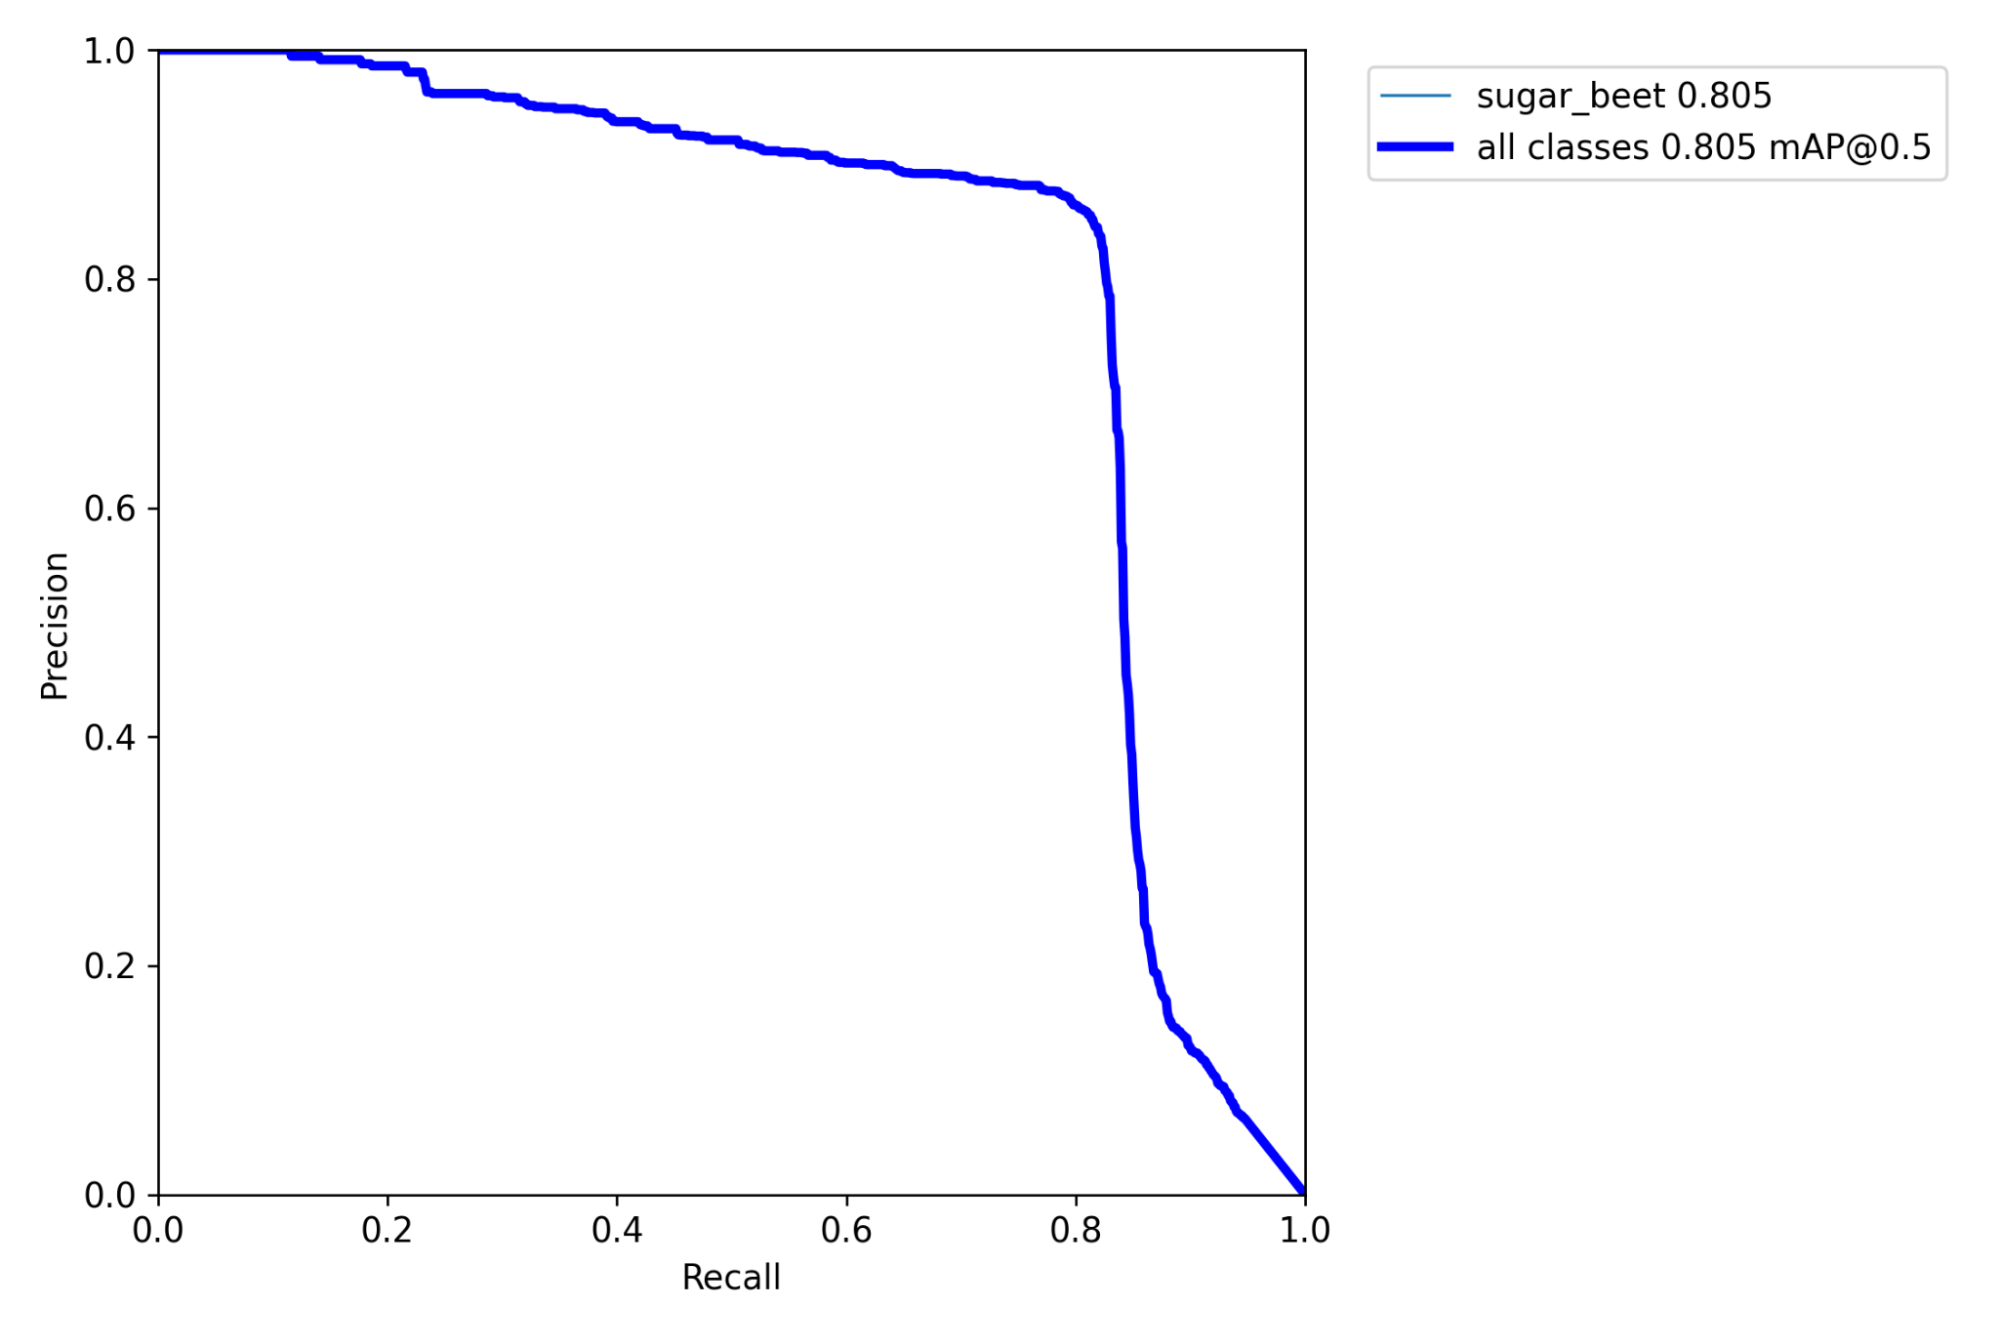
\includegraphics[scale=0.1]{figures/comp_medium.png}
	\caption{Comparison of small and medium sized model. Left one (small model) has AUC of 0.806 and right one (medium) AUC of 0.805.}
	\label{fig:comparison_small_medium}
\end{figure}

Both R-P-curves look quite similar. However, the left one (small model) has a bit smaller precision in regions of small recall. In contrast, with higher recall, the small model has higher precision. All in all, both models have similar AUC with $ 0.806 $ (small) and $ 0.805 $ (medium). This small difference and the fact that the small model has much faster inference times lead to the decision to not further train the medium model and focus on the small one. \\

With the knowledge of the large model to include background images and use higher data augmentation, the setting of the small model can also be adjusted accordingly. With these hyperparameters and a pretrained model on the sugar beet images labeled as whole picture as one plant, the following results of figure \ref{fig:result_small_one} can be observed. 

\begin{figure}[htb!]
	\centering
	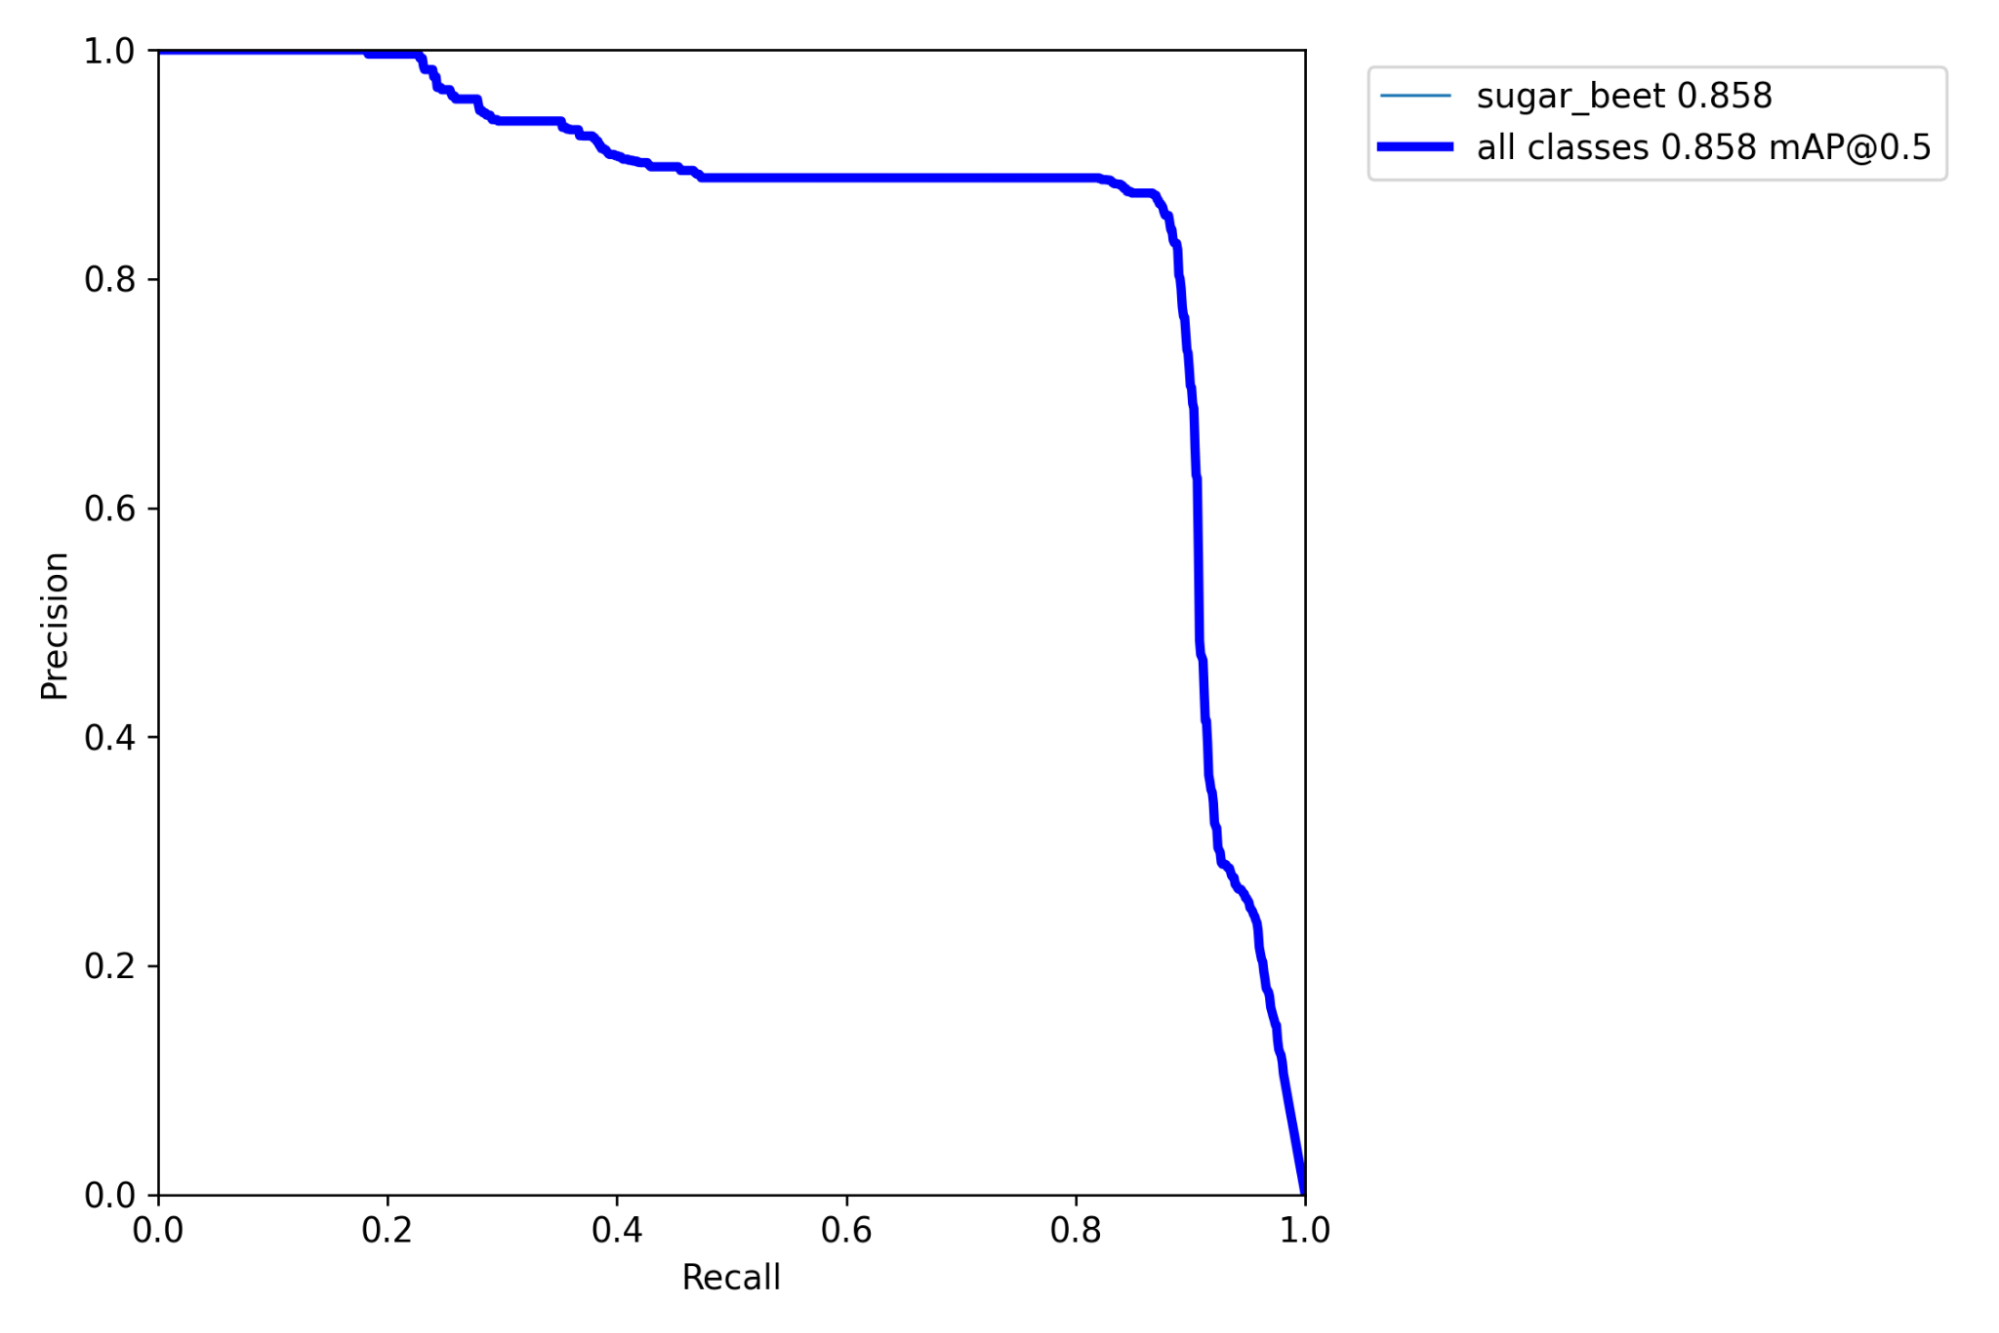
\includegraphics[scale=0.12]{figures/result_small.png}
	\caption{Result of the better trained small model. Now, the average precision is 0.858.}
	\label{fig:result_small_one}
\end{figure}

It can be seen that the accuracy has further improved compared to the first experiments. Now, with small recall (nearly up to 0.3), a precision of about $ 100\% $ can be achieved. The curve now drops much faster, but later. The overall AUC is increased by approximately $ 6\% $ and lays at $ 0.858 $.

\section{Comparison and Discussion}
In this section, a comparison is made and a general discussion about the models introduced and the object detection in general is presented.

Now the first aspect is the type of model. YOLO is in general very efficient due to the architecture and the idea of processing the image once (\"you only look once\"). However, in the real time application of detecting the plants in the field, big differences between the large and small architectures can be observed. While the large model takes nearly half a second per image, the small one can predict the labels of a videostream nearly 10 times per second. This makes it very hard to apply the model in-place in the mobile application as it would not be very user-friendly.

One next aspect is the accuracy of predicted labels. While the large model has an AUC of $ 87.2\% $, the small model has an AUC of $ 85.8\% $. As expected, the larger models predicts the bounding boxes of sugar beets in fields more accurately. But the difference to the small model is very low. We also have to keep in mind that about $ 10000 $ images of sugar beets were labeled manually. Of course, this was done as exactly as possible, but in many cases, the borders of sugar beets were not clearly visible at first or even second glance leading to small errors in the labeling. Especially in images of larger sugar beet plants, the bounding box labeling by hand is very hard because of the overlapping leafs. Especially with this background, the small difference of accuracy between large and small model is not too important.\\

All in all, this leads to the decision of implementing the small model directly in the application. It has two advantages. The first is that the user can directly see if a plant is detected and immediately adjust the camera position and angle. Another possibility is the implementation of adjusting the bounding box so that a different part of the image is cropped if the user thinks that the prediction is not correct enough. This leads to more flexibility of the application. 

The following images show results of detected sugar beets. They can be seen in figure \ref{fig:final_results} and some properties of the model can be followed. The first two examples (figure \ref{fig:result_1} and \ref{fig:result_2}) show easier cases. Image \ref{fig:result_1} is already very similar to the standardized format. The camera angle is $ 90° $ and the plant is centered. The second one \ref{fig:result_2} depicts small plants where the boundaries do not overlap and the soil has a completely different color than the plants which makes the detection easier. Example \ref{fig:result_3} shows an edge case. It shows two half plants at the top and right border of the image. They have high damage and are not centered on the image. However, one sugar beet plant is detected at the top of the picture because the structure of the plant was learned. In this case, the live application in the app helps the user to find the right position of the camera. He would have to move it to the top to capture the whole plant. In figures \ref{fig:result_4} and \ref{fig:result_5}, many larger plants are depicted. In the first one (\ref{fig:result_4}), 5 plants are detected with low confidence because it is very hard to find the borders because of the overlaps. However also in this case, the user of the app can use this information to hold the camera closer to the field. In the last image \ref{fig:result_5}, two plants are detected with higher confidence. Especially the upper one can be detected very well because the boundaries can be seen much better than all other sugar beets in this picture. Additionally, the source of the leafs can be seen here which makes it easier to center the bounding box on the plant. This is a tendency that can be observed for the whole model. If this is the case, the bounding box is much better than in cases of leafs not being structured.

\begin{figure}[htb!]
	\begin{subfigure}{.4\textwidth}
		\centering
		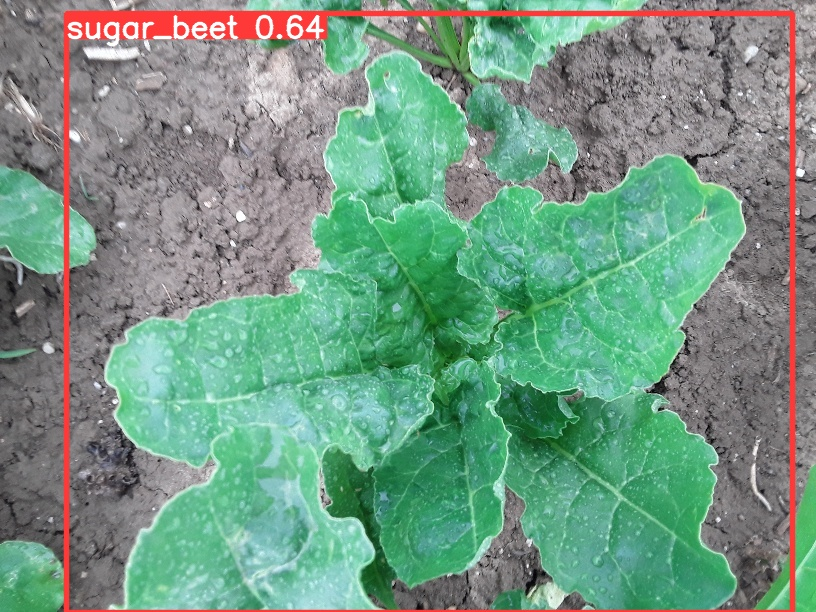
\includegraphics[scale=0.19]{figures/result_1.jpg}
		\caption{Example of an image with only one plant. The image is already similar to the standardized format.}
		\label{fig:result_1}
	\end{subfigure}%
	\begin{subfigure}{.6\textwidth}
		\centering
		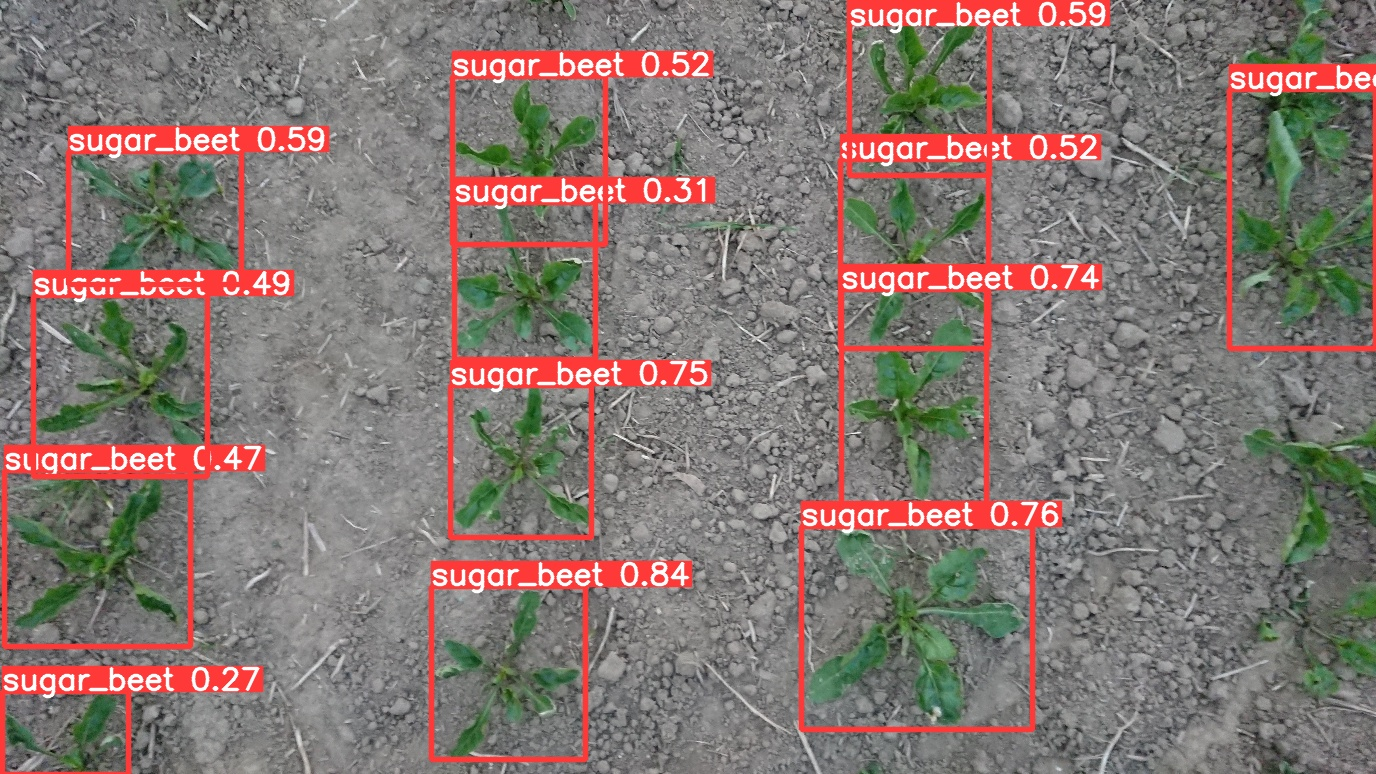
\includegraphics[scale=0.15]{figures/result_2.JPG}
		\caption{Example of many small plants. The model is able to predict the boundaries very well because of nearly no overlap between the sugar beets.}
		\label{fig:result_2}
	\end{subfigure}
	\begin{subfigure}{.4\textwidth}
		\centering
		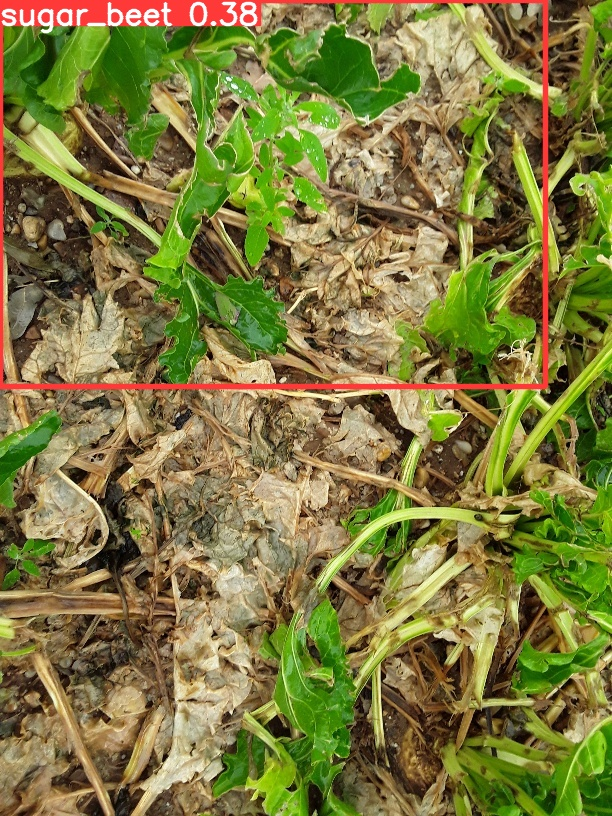
\includegraphics[scale=0.2]{figures/result_3.jpg}
		\caption{Example of an image of plants with high damage. The picture was not taken optimally (angle, not centered on one plant). The model detects one plant at the top of the image.}
		\label{fig:result_3}
	\end{subfigure}
	\begin{subfigure}{.6\textwidth}
		\centering
		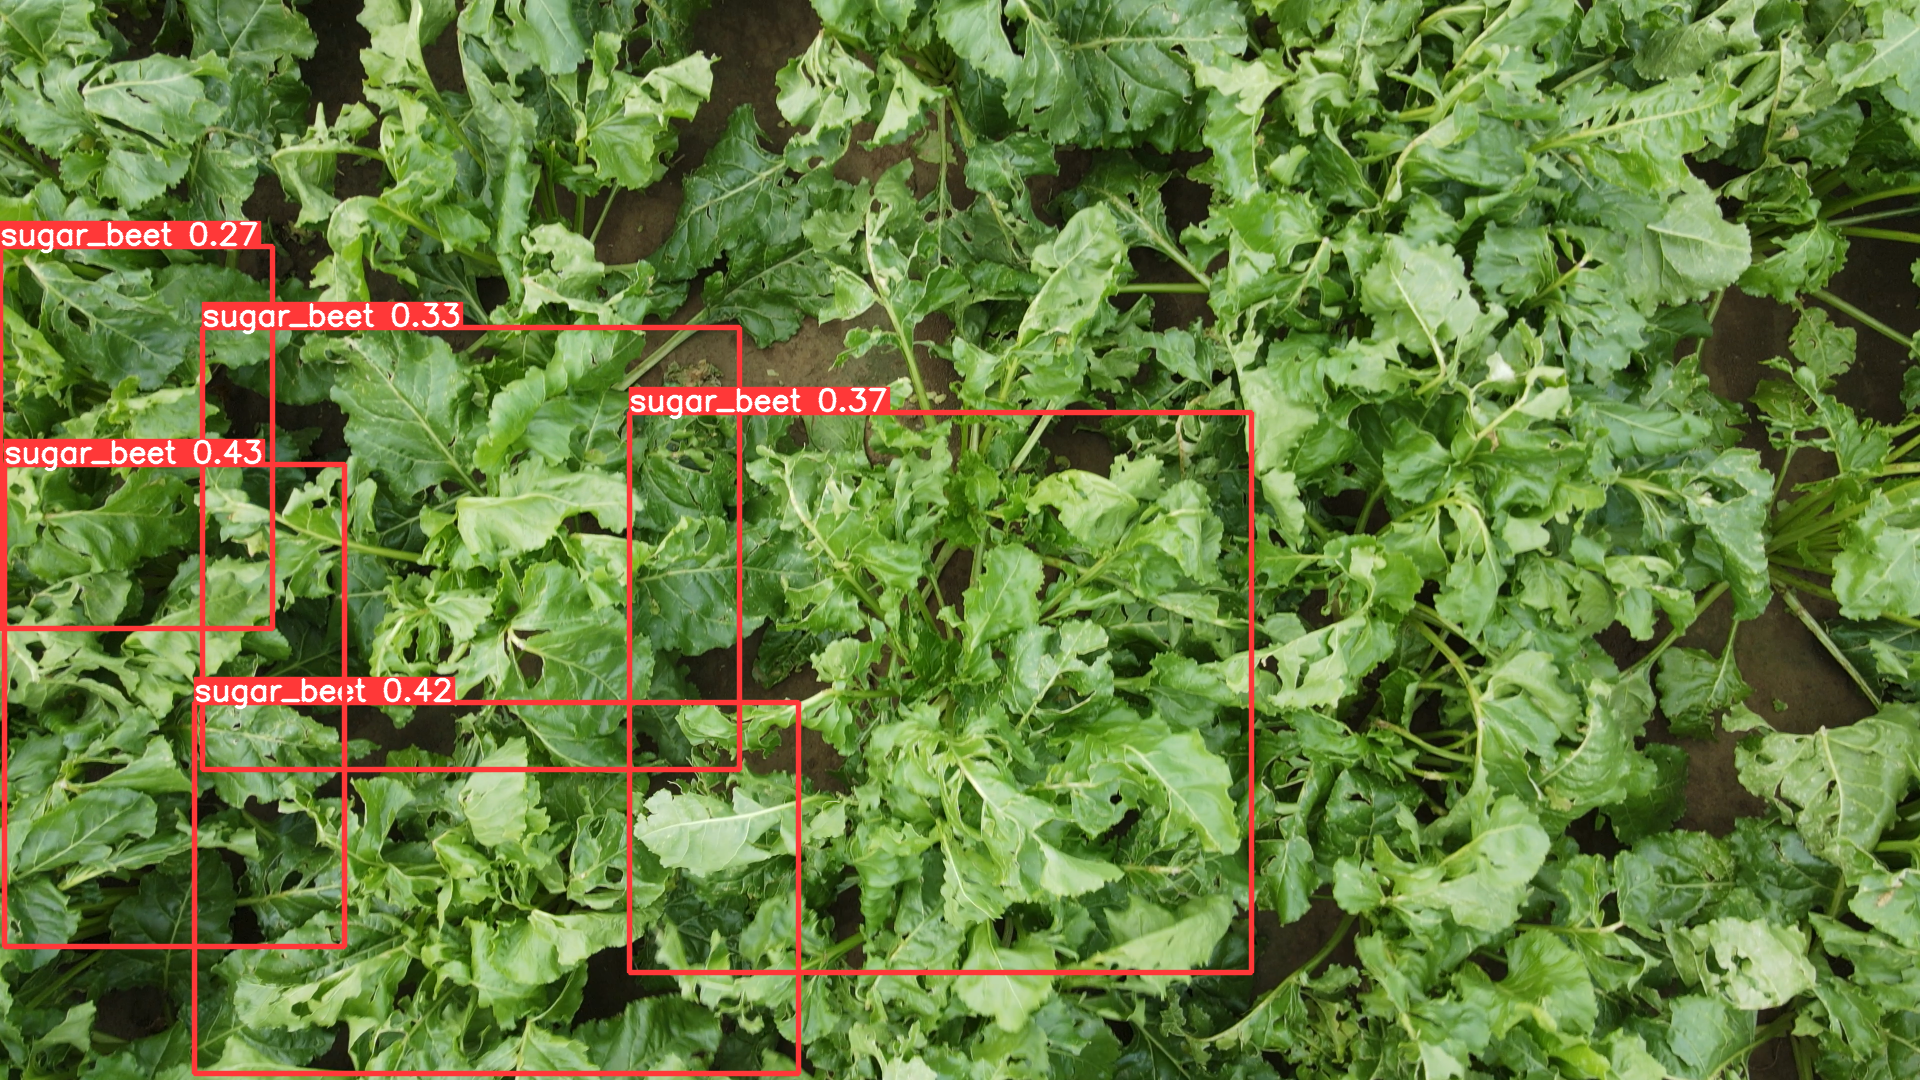
\includegraphics[scale=0.115]{figures/result_4.png}
		\caption{Example of many larger plants. The model detects 5 sugar beet plants with relatively low confidence because the boundaries can not be seen very easily.}
		\label{fig:result_4}
	\end{subfigure}
	\begin{subfigure}{1\textwidth}
		\centering
		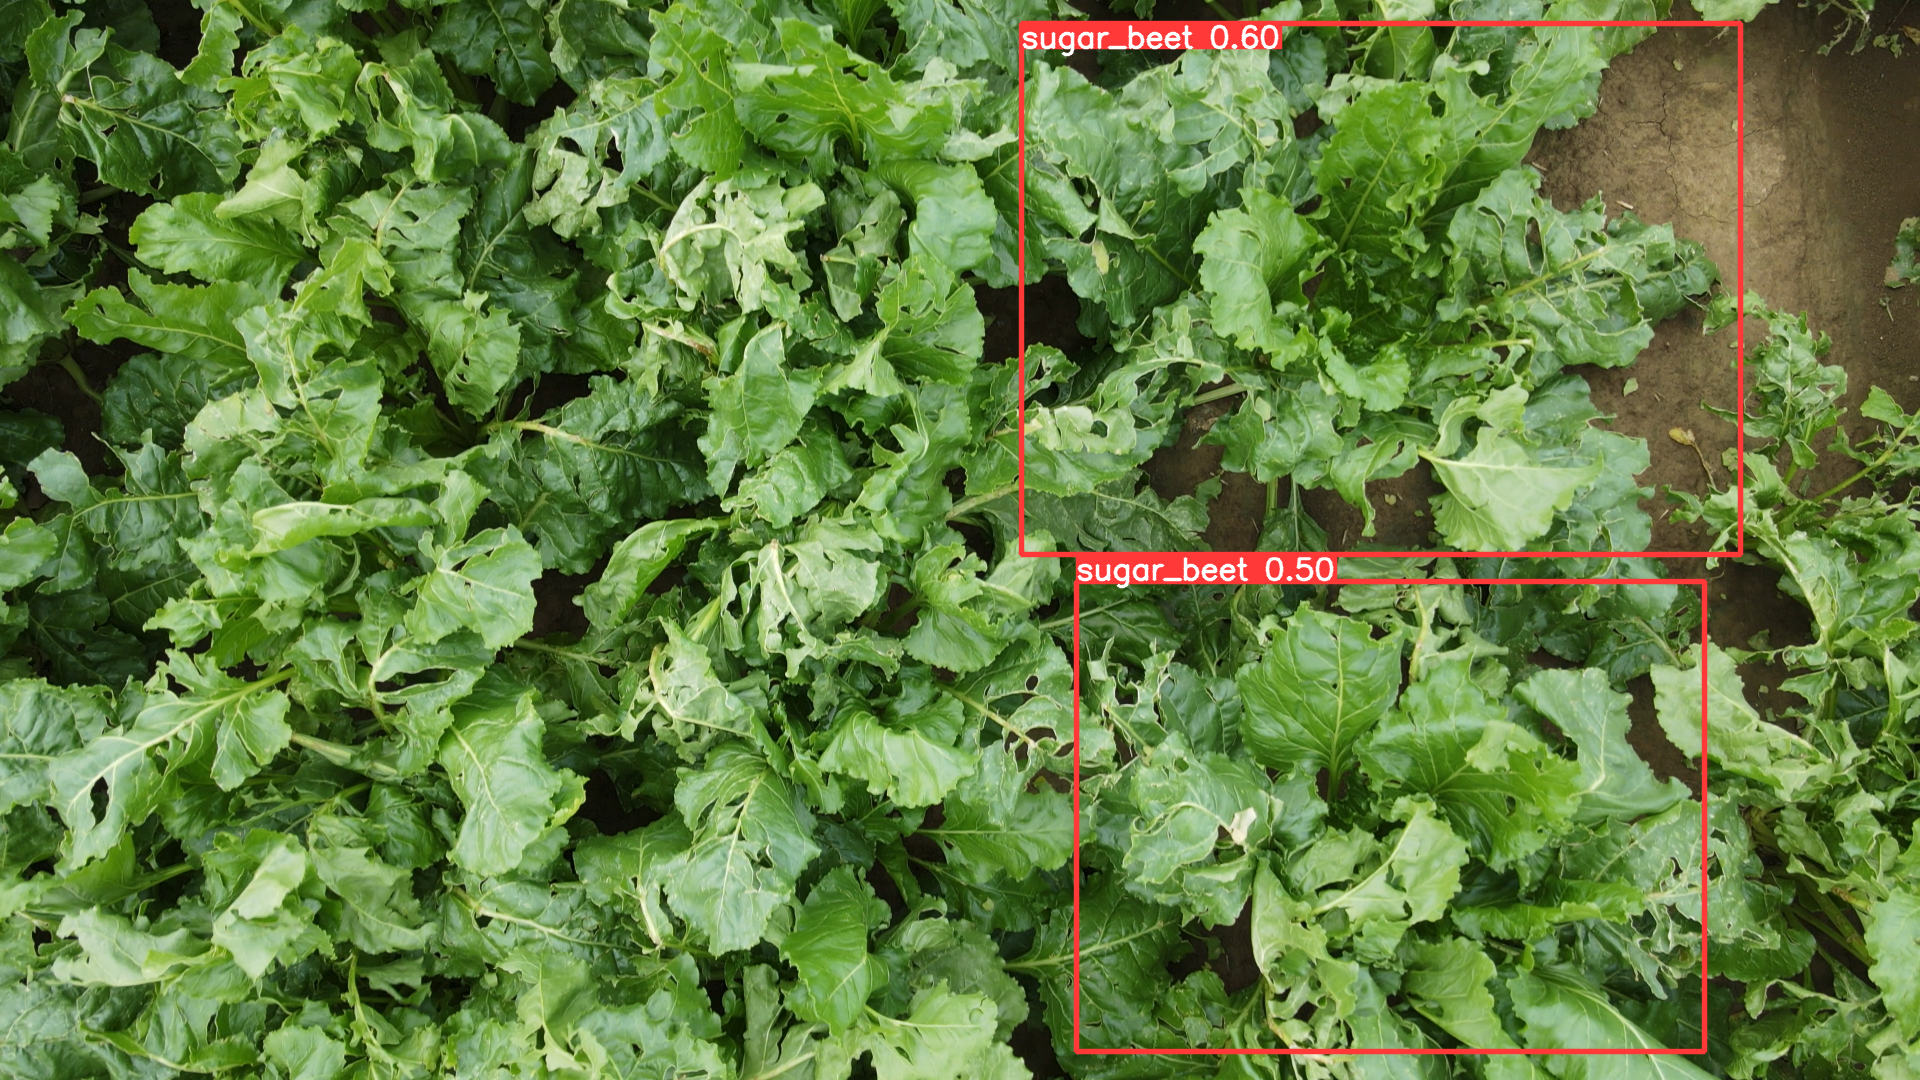
\includegraphics[scale=0.115]{figures/result_5.png}
		\caption{Example of many larger plants. The model detects 2 sugar beet plants. The upper one with higher confidence because the boundaries are clearer there.}
		\label{fig:result_5}
	\end{subfigure}
	\caption{Results of the object detection algorithm. Different scenarios are tested.}
	\label{fig:final_results}
\end{figure}
